% TeX source
%
% Author: Tetsuya Ishikawa <tiskw111@gmail.com>
% Date  : March 01, 2020
%%%%%%%%%%%%%%%%%%%%%%%%%%%%%%%%%%%%%%%%%%%%%%%%%%%%% SOURCE START %%%%%%%%%%%%%%%%%%%%%%%%%%%%%%%%%%%%%%%%%%%%%%%%%%%%%

\subsection{実確率変数の期待値}

突然ではあるが,確率変数の期待値について簡単に説明をさせて頂きたい.
まずは簡単のため,集合$\{z_1, z_2, \ldots, z_I \}$上のいずれかの値を取る離散確率変数$Z$を考える.
この確率変数$Z$の期待値は
\begin{equation}
    \mathrm{E}[X] = \sum_{i = 1}^{I} p_i z_i,
\end{equation}
で与えられる.ただし$p_i$は$Z$が値$z_i$を取る確率である.
連続確率変数でも同じことが言える.確率変数$X$をとある確率空間上で可測な実数値確率変数とし,
$X$が実数値$x$を取る確率密度関数を$p(x)$とおく.このとき確率変数$X$の期待値は
\begin{equation}
    \mathrm{E}[X] = \int_{\mathbb{R}} p(x) x \, \mathrm{d}x,
    \label{eqn:random_variable_expectation}
\end{equation}
で与えることができる.まさに離散確率変数の期待値を連続化したような式になっている.
ちなみに確率変数$X$が$M$次元のベクトル確率変数であった場合は
\begin{equation}
    \mathrm{E}[X] = \idotsint_{\mathbb{R}} p(\bs{x}) \bs{x}
    \, \mathrm{d}x_1 \cdots \mathrm{d}x_M,
    \label{eqn:random_variable_expectation_multi_dim}
\end{equation}
となる.

さらに,式(\ref{eqn:random_variable_expectation})の右辺を解析的に解くことが困難であったとしよう.
このとき我々には何が出来るであろうか.そう,期待値なのであるから,実際に確率変数$X$をいくつか生成してみて,
その平均値をもって期待値の近似値とすることができる.これはいわゆるMonte Carlo法であり,数式で表現すると
\begin{equation}
    \mathrm{E}[X] \approx \frac{1}{L} \sum_{\ell = 1}^{L} X_{\ell},
\end{equation}
となる.ただし$X_{\ell}$は確率変数$X$のサンプリングである.

何でいきなりこんな話をしたかって?
マァマァ,黙って式(\ref{eqn:random_variable_expectation}), (\ref{eqn:random_variable_expectation_multi_dim})
を目に焼き付けておいて頂きたい.

\subsection{カーネルのFourier変換}

さて,本題のRFFに話を戻そう.
以下ではカーネル関数$k(\bs{x}, \bs{y})$を$k(\bs{x} - \bs{y})$と表現できるものだけに限定しよう.
多項式カーネルやFisherカーネルなど多くの有名なカーネル関数が議論の対象外になってしまうものの,
式(\ref{eqn:kernel_rbf})で与えられるRBFカーネルは幸いにも$k(\bs{x} - \bs{y})$はそのように書き表すことができる.

さて,カーネル関数$k(\bs{x} - \bs{y})$をFourier変換し,その結果を$p(\bs{\omega})$と置いてみよう.すなわち
\begin{align}
    p(\bs{\omega})
    &= \mathcal{F} [k](\bs{\omega}) \notag \\
    &= \idotsint_{\mathbb{R}^M} k(\bs{z}) e^{-i\bs{\omega}\tran\bs{z}} \, \mathrm{d}z_1 \cdots \mathrm{d}z_M,
    \label{eqn:fourier_of_kernel}
\end{align}
である.これを逆Fourier変換を用いて$k(\bs{x} - \bs{y}) = \cdots$の形に書き直すと
\begin{align}
    k(\bs{x} - \bs{y})
    &= \mathcal{F}^{-1} [p](\bs{x} - \bs{y}) \notag \\
    &= \idotsint_{\mathbb{R}^M} p(\bs{\omega}) e^{i\bs{\omega}\tran(\bs{x} - \bs{y})} \, \mathrm{d}\omega_1 \cdots \mathrm{d}\omega_M,
    \label{eqn:inv_fourier_of_kernel}
\end{align}
が成り立つ.これは逆Fourier変換の定理から明らかであろう.

さて,式(\ref{eqn:inv_fourier_of_kernel})を見て思うことはないだろうか.
そう,期待値である.つまり$p$を確率密度関数とみなせば
\begin{equation}
    k(\bs{x} - \bs{y}) = \mathrm{E}_{\bs{\omega} \sim p} \left[ e^{i\bs{\omega}\tran(\bs{x} - \bs{y})} \right],
    \label{eqn:rff_expectation}
\end{equation}
と表すことができる.
ただし,上式の期待値は$\bs{\omega}$を確率変数とみなし,
さらにその確率分布は確率密度関数$p(\bs{\omega})$に従うとみなしていることに注意せよ.
期待値記号$\mathrm{E}$の添字に${\bs{\omega} \sim p}$を書いたのは,そのことを明記するためである.

先に指摘した通り,我々は期待値計算をMonte Carlo法で近似できることを知っている.
確率密度関数$p(\bs{\omega})$にしたがって確率変数$\bs{\omega}$をサンプリングした値を
$\{\bs{\omega}_\ell\}_{\ell=1}^{L}$とすると,
\begin{align}
    k(\bs{x} - \bs{y})
    &= \mathrm{E}_{\bs{\omega} \sim p} \left[ e^{i\bs{\omega}\tran(\bs{x} - \bs{y})} \right]
    \notag \\
    &\approx \frac{1}{L} \sum_{\ell = 1}^{L} e^{i\bs{\omega}_\ell\tran(\bs{x} - \bs{y})},
    \label{eqn:rff_approx}
\end{align}
が成り立つのである.
これにより,カーネル関数を,Fourier変換と乱数を用いて近似できたことになる.これがRFFの本質である.

さて,興奮に任せて大切なポイントをひとつ取り落してしまったことは読者もお気付きであろう.
式(\ref{eqn:rff_expectation})が成立するためには,関数$p(\bs{\omega})$が確率密度関数と同格でなければならない.
すなわち,可積分かつ非負の値を取る関数でなければならない.
しかし驚くべきことに,カーネル関数が正定値関数である限り,そのFourier変換は可積分かつ非負であることが証明できる.
これは非常に大事な事実であるから,定理としてまとめておく.ただし,議論の流れを妨げないよう証明は本文書の最後の節で行う.

\begin{theorem}[平行移動不変な正定値カーネルのFourier変換]
    正定値カーネル関数$k(\bs{x}, \bs{y})$が平行移動不変,すなわち$k(\bs{x}, \bs{y}) = k_{\Delta}(\bs{x} - \bs{y})$
    をみたす関数$k_{\Delta}$が存在したとする.このとき,カーネル関数$k_{\Delta}(\bs{x} - \bs{y})$のFourier変換は
    $L_1$ノルムの意味で可積分であり,かつ非負関数である.
\end{theorem}

さて,最後に近似したカーネル関数をどのように使うかについて説明しよう.
一般に,カーネル関数は正定値関数であるから,式(\ref{eqn:rff_approx})の最右辺の虚部は不要である.したがって
\begin{align}
    k(\bs{x} - \bs{y})
    &\approx \frac{1}{L} \sum_{\ell = 1}^{L} e^{i\bs{\omega}_\ell\tran(\bs{x} - \bs{y})}
    \label{eqn:rff_feature_expand_1} \\
    &= \frac{1}{L} \sum_{\ell = 1}^{L} \cos (\bs{\omega}_\ell\tran(\bs{x} - \bs{y}))
    \label{eqn:rff_feature_expand_2} \\
    &= \frac{1}{L} \sum_{\ell = 1}^{L} \bigl[
        \cos (\bs{\omega}_\ell\tran\bs{x}) \cos (\bs{\omega}_\ell\tran\bs{y}) \notag \\
    &\hspace{60pt} + \sin (\bs{\omega}_\ell\tran\bs{x}) \sin (\bs{\omega}_\ell\tran\bs{y}) \bigr],
    \label{eqn:rff_feature_expand_3}
\end{align}
を得る.ただし式(\ref{eqn:rff_feature_expand_1})から式(\ref{eqn:rff_feature_expand_2})へはEulerの公式を,
式(\ref{eqn:rff_feature_expand_2})から式(\ref{eqn:rff_feature_expand_3})へはかの懐しき三角関数の加法定理を用いた.
さてここでベクトル
\begin{equation}
    \bs{u}(\bs{x}) \triangleq \frac{1}{\sqrt{L}}
    \begin{pmatrix}
        \cos (\bs{\omega}_1\tran\bs{x}) \\
        \vdots \\
        \cos (\bs{\omega}_L\tran\bs{x}) \\[5pt]
        \sin (\bs{\omega}_1\tran\bs{x}) \\
        \vdots \\
        \sin (\bs{\omega}_L\tran\bs{x})
    \end{pmatrix}
    =
    \begin{pmatrix}
        \cos (\bs{W}\bs{x}) \\[2pt]
        \sin (\bs{W}\bs{x})
    \end{pmatrix}
    \label{eqn:rff_transform}
\end{equation}
を導入しよう.
ただし行列$\bs{W} = (\bs{\omega}_1, \ldots, \bs{\omega}_L)\tran$であり,
上式の最右辺ではベクトルの余弦関数を$\cos \bs{x} = (\cos x_1, \ldots, \cos x_L)\tran$と定義して使用している.
$\sin$についても同様である.
すると式(\ref{eqn:rff_feature_expand_3})の右辺は
\begin{equation}
    \bs{u}(\bs{x})\tran \bs{u}(\bs{y}),
\end{equation}
と非常にシンプルに書き改めることができる.すなわち
\begin{equation}
    k(\bs{x} - \bs{y}) \approx \bs{u}(\bs{x})\tran \bs{u}(\bs{y}),
    \label{eqn:rff_final}
\end{equation}
と近似することができたのである.

そもそもカーネル関数は,特徴量の内積であったことを思い出してほしい.
式(\ref{eqn:rff_final})は,カーネル関数を近似することと,
特徴量として$\phi_{\bs{x}}$ではなく$\bs{u}(\bs{x})$を使うことが等価だと言っているのである.
つまり図\ref{fig:rff_and_feature_extraction}のような構図が成り立つ.

\begin{figure}[t]
    \centerline{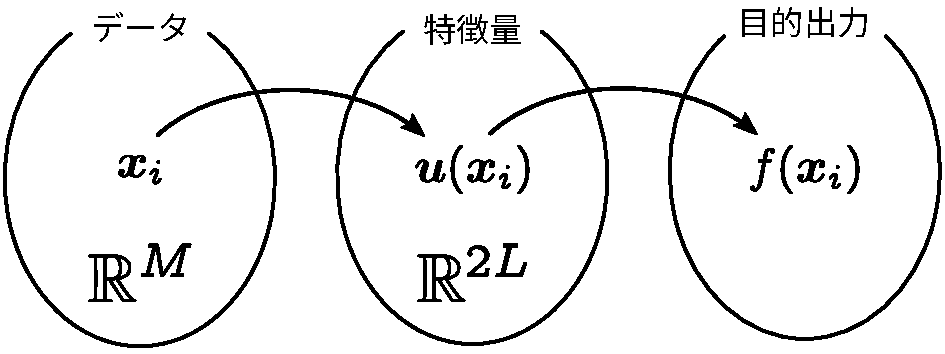
\includegraphics[width=200pt]{figures/rff_and_feature_extraction.pdf}}
    \caption{RFFと特徴抽出}
    \label{fig:rff_and_feature_extraction}
\end{figure}

今,特徴量はもはや関数ではなく,ただの$2L$次元の実ベクトルである.
したがって,回帰や分類などのタスクを実行するのにミョーチクリンなトリックはもはや必要ない.
有限次元の線形回帰なり線形サポートベクターマシンなりを適用すれば良いのである.
線形サポートベクターマシンの学習および推論は,カーネルサポートベクターマシンと比較すると桁違いに速い.
しかも特徴量は,高々有限次元の近似とはいえ,カーネル関数の柔軟性を残している.
このようにしてカーネル法はその柔軟性を残しつつ大規模データに適用しうるだけの高速性を手にすることができるのである.

\subsection{RBFカーネルの場合}

さて,実際にRFFを運用するためには,カーネル関数を何らかの関数に定め,
そのカーネル関数に対して確率密度関数$p(\bs{\omega})$を算出しなければならない.
RFFはカーネル関数が$k(\bs{x} - \bs{y})$と表現できるものに限られるから,ここではRBFカーネルの場合について考察しよう.

とはいえ,確率密度関数$p(\bs{\omega})$の導出は式(\ref{eqn:fourier_of_kernel})にしたがってFourier変換を
計算するだけである.直接計算だけであるので証明は省略するが,
\begin{equation}
    p(\bs{\omega}) = \frac{1}{\sqrt{2 \pi \sigma^2}^{M}} \exp \left( - \frac{\| \bs{\omega} \|^2}{2 \sigma^2} \right),
\end{equation}
となる.つまり確率変数$\bs{\omega}$は正規分布するのである.
したがって確率変数$\bs{\omega}$は正規分布からサンプリングすれば良いということになる.

以上をまとめると,RBFベースのRFFは次の手順で実施すれば良い.
\begin{enumerate}
    \item RFFの自由度$L \in \mathbb{Z}^{+}$を適当な数に設定する.これはカーネル関数を近似する際のサンプリング数である.
    \item 行列の各要素が正規分布にしたがうランダム行列$\bs{W} \in \mathbb{R}^{L \times M}$を生成する.
    \item 各学習データ$\bs{x}_i$に式(\ref{eqn:rff_transform})の変換を施し,それを改めて学習データセットとみなす.
    \item 変換後のデータセットに対し,線形回帰や線形サポートベクターマシンなどのアルゴリズム$f$を適用する.
    \item 推論時には,推論データ$\bs{x}$に対してもデータ変換式(\ref{eqn:rff_transform})を適用して$\bs{u}(\bs{x})$を算出し,
          その後に推論$f(\bs{u}(\bs{x}))$を行う.
\end{enumerate}

\subsection{数値実験:RBFカーネルのRFF近似}

本節では,RFFを用いてRBFカーネルが近似される様子を実際に確認してみよう.
まずは近似前のRBFカーネルを
\begin{equation}
    k(x_1, x_2) \triangleq \exp \left(- \frac{\| x_1 - x_2 \|^2}{2} \right),
\end{equation}
とおくとしよう.このとき対応するRFFの確率密度関数は
\begin{equation}
    p(\omega) = \frac{1}{\sqrt{2 \pi}} \exp \left(- \frac{\| \omega \|^2}{2} \right),
\end{equation}
となるので,RFF近似したRBFカーネルは
\begin{equation}
    k_{\textrm{rff}}(x_1, x_2) \triangleq \bs{u}(x_1)\tran \bs{u}(x_2),
    \hspace{10pt}
    \omega_1, \ldots, \omega_L \sim p(\omega),
\end{equation}
となる.これを試みに$L = 10, 100, 1000$として描画してみたのが図\ref{fig:rff_approximation}である.
RFFの次元を上げるにつれてRBFカーネルに近づいていくことが分かるであろう.

\begin{figure*}[t]
    \centerline{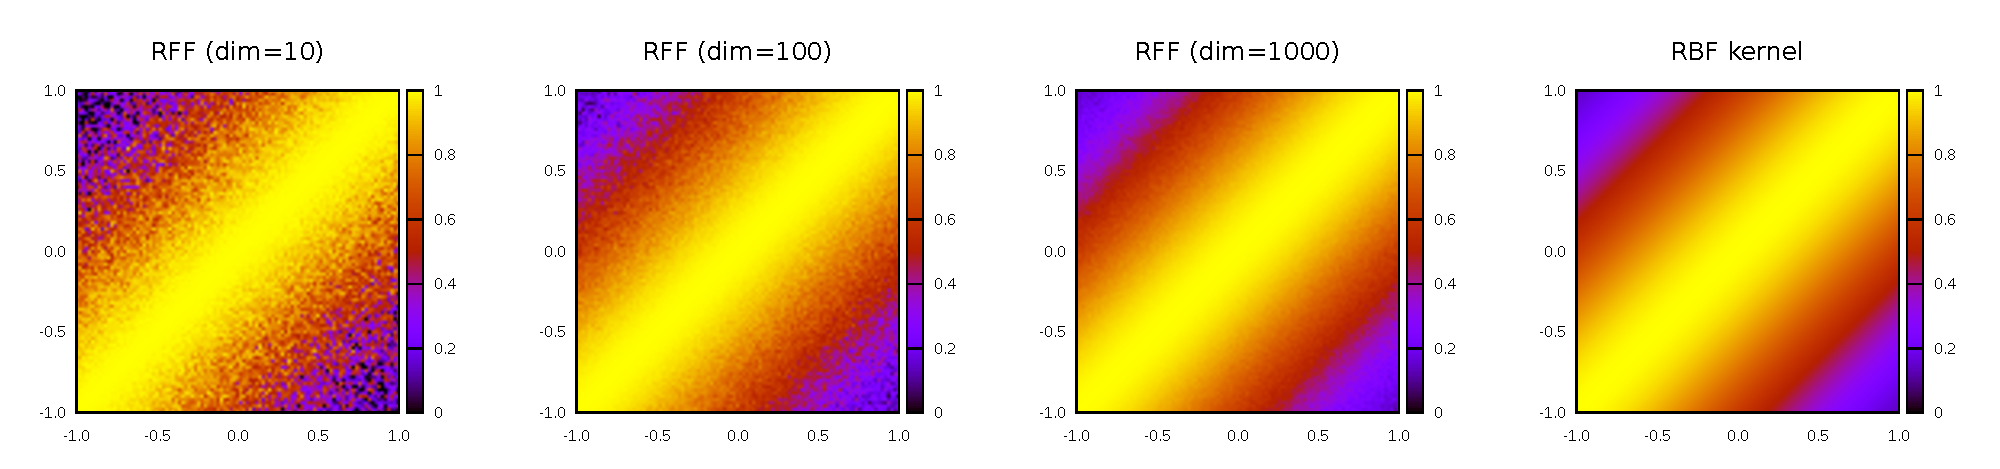
\includegraphics[width=540pt]{figures/kernel_approximation.pdf}}
    \caption{RBFカーネルのRFF近似}
    \label{fig:rff_approximation}
\end{figure*}

\subsection{深層学習との関係}

最後に,RFFを用いたサポートベクターマシンと深層学習との関係性について述べておく.
RFFは入力データ$\bs{x}$の特徴量を式(\ref{eqn:rff_transform})で定める手法であった.
これを線形サポートベクターマシンと組み合わせてみよう.

問題設定としては,教師付き学習データを用いて$C$クラスのクラス分類器を作成することを目標としよう.
学習データセットは$\mathcal{D} = \{ (\bs{x}_n, y_n) \}_{n=1}^{N}$とする.
ただし$\bs{x}_n \in \mathbb{R}^M$, $y_n \in \{1, 2, \ldots, C\}$であり,
$\bs{x}_n$が学習データに,$y_n$が教師データに対応する.

さて,線形サポートベクターマシンの判別式は線形関数であるから,
入力データ$\bs{x}$に対する各クラスの対数尤度は
\begin{equation}
    f_c(\bs{x}) = \bs{a}_c\tran \bs{x} + b_c,
    \label{eqn:rff_svm_class_wise}
\end{equation}
で表現される.ベクトル$\bs{a}_c$およびスカラー$b_c$は学習パラメータであり,各クラスの対数尤度を上手く表現できるように学習される.

さて,少しだけ表現を変更しよう.まず,すべてのクラスをまとめて記述するために,
$\bs{A} = (\bs{a}_1, \ldots, \bs{a}_C)\tran$, $\bs{b} = (b_1, \ldots, b_C)$とおく.
さらに,RFFの適用を前提とすれば,入力データは$\bs{x}$ではなく$\bs{u}(\bs{x})$に置き換えなければならない.
すると式(\ref{eqn:rff_svm_class_wise})は
\begin{equation}
    \bs{f}(\bs{x}) = \bs{A}
    \begin{pmatrix}
        \cos(\bs{Wx}) \\ \sin(\bs{Wx})
    \end{pmatrix}
    + \bs{b},
\end{equation}
となる.

これを深層学習の立場から見ると,ちょっと特殊な活性化関数を用いた,
2層の全結合層を持つニューラルネットワークとみなすことができる.
図\ref{fig:rff_svc_as_dnn}を参照されたい.

\begin{figure*}[t]
    \centerline{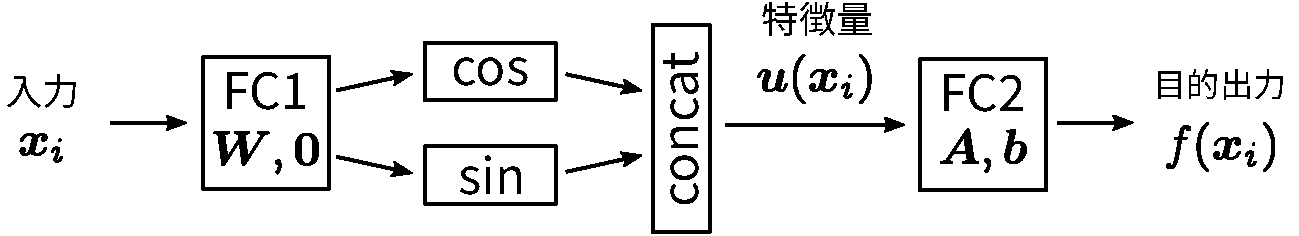
\includegraphics[width=350pt]{figures/rff_svc_as_dnn.pdf}}
    \caption{RFFとニューラルネットワーク}
    \label{fig:rff_svc_as_dnn}
\end{figure*}

もちろん,学習の仕方はサポートベクターマシンと深層学習で全く異なることに注意されたい.
サポートベクターマシンは区分的線形な目的関数を制約付き2次計画問題に帰着させているのに対し,
深層学習ではクロスエントロピーを確率的勾配法で最小化させている.

%%%%%%%%%%%%%%%%%%%%%%%%%%%%%%%%%%%%%%%%%%%%%%%%%%%%% SOURCE FINISH %%%%%%%%%%%%%%%%%%%%%%%%%%%%%%%%%%%%%%%%%%%%%%%%%%%%
% vim: expandtab tabstop=4 shiftwidth=4 fdm=marker
